\section{Интерпретатор языка BASIC}
\label{sec:basic_interpreter}

В данном разделе мы рассмотрим интерпретатор языка Basic. Это программа, которая 
выполняет другие программы написанные на языке Basic. Конечно, мы ограничимся 
лишь частью команд этого языка, наш интерпретатор будет распознавать следующие 
команды:

\begin{description}
	\item[PRINT] {\it выражение}

	Выводит результат вычисления выражения.

	\item[INPUT] {\it переменная}

	Выводит {\it приглашение} на экран (?), ожидает ввод целого числа с 
клавиатуры и затем присваивает это число переменной.

	\item[LET] {\it переменная = выражение}

	Присваивает переменной результат вычисления выражения.

	\item[GOTO] {\it номер строки}

	Выполнение продолжится с указанной строки.

	\item[IF] {\it условие} {\bf THEN} {\it номер строки}

	Выполнение продолжится с указанной строки если условие верно.
	
	\item[REM] {\it строка символов}

	Комментарии.
\end{description}

Каждая строка программы Basic помечена номером и содержит лишь одну инструкцию. 
Программа, вычисляющая факториал для числа введённого с клавиатуры, выглядит 
следующим образом:

\begin{lstlisting}[language={[Visual]Basic}]
 5  REM inputting the argument
10  PRINT " factorial of:"
20  INPUT A
30  LET B = 1 
35  REM beginning of the loop
40  IF A <= 1 THEN 80 
50  LET B = B * A
60  LET A = A - 1
70  GOTO 40 
75  REM prints the result
80  PRINT B
\end{lstlisting}

Реализуем также мини–редактор по принципу интерактивного цикла. У нас должна 
быть возможность добавлять новые строки, вывод программы и её вычисление. 
Запуск предыдущей программы осуществляется командой \code{RUN}. Пример 
вычисления этой программы.

\begin{lstlisting}
> RUN
 factorial of: ? 5
120
\end{lstlisting}

Это вычисление можно разбить на несколько разных этапов.

\begin{description}
	\item[Описание абстрактного синтаксиса]

	необходимо определить типы данных для описания программ на Basic, а так же 
другие компоненты (строки, комментарии, выражения, и т.д.)

	\item[Вывод программы]

	эта часть состоит в переводе программы на Basic из внутреннего формата в 
строки, для того чтобы вывести ее на экран.

	\item[Лексический и синтаксический анализ]

	обе эти части проделывают обратную операцию, то есть перевод строки во 
внутренний формат программы на Basic (абстрактный синтаксис)

	\item[Вычисление]

	это основа интерпретатора. Далее мы увидим что функциональный язык как 
Objective CAML особенно хорошо подходит для решения подобных проблем.

	\item[Интерактивный цикл]

	здесь реализуется все вышесказанное.
\end{description}

\subsection{Абстрактный синтаксис}
\label{subsec:abstract_syntax}

% TODO переделать по-нормальному
\begin{verbatim}
Unary_Op        ::=     -    |    !
Binary_Op       ::=     +    |    -    |    *    |    /    |    %
        |       =    |    <    |    >    |    <=    |    >=    |    <>
        |       &    |    ' | '
Expression      ::=     integer
        |       variable
        |       "string"
        |       Unary_Op   Expression
        |       Expression   Binary_Op   Expression
        |       ( Expression )
Command         ::=     REM string
        |       GOTO integer
        |       LET variable = Expression
        |       PRINT Expression
        |       INPUT variable
        |       IF Expression THEN integer
 
Line    ::=     integer Command
 
Program         ::=     Line
        |       Line Program
 
Phrase  ::=     Line | RUN | LIST | END
\end{verbatim}

Заметим, что правильность выражения с точки зрения грамматики не означает 
возможность его вычисления. Например, \code{1 + ``hello''} есть выражение, 
однако его невозможно вычислить. Это сделано с целью облегчить абстрактный 
синтаксис языка Basic. Расплата за это --- программы на Basic, синтаксически 
правильные, могут привести к ошибке из--за несоответствия типов.

Теперь определить типы данных Objective CAML просто, достаточно перевести 
абстрактный синтаксис в тип сумма.

\begin{lstlisting}[language=OCaml]
# type op_unr = OPPOSE | NON  ;;
# type op_bin = PLUS | MOINS | MULT | DIV | MOD  
             | EGAL | INF | INFEQ | SUP | SUPEQ | DIFF 
             | ET | OU  ;;
# type expression = 
     ExpInt of int 
   | ExpVar of string
   | ExpStr of string 
   | ExpUnr of op_unr * expression
   | ExpBin of expression * op_bin * expression  ;;
# type instruction = 
     Rem of string
   | Goto of int 
   | Print of expression
   | Input of string 
   | If of expression * int 
   | Let of string * expression  ;;
# type ligne = { num : int ; inst : instruction }  ;;
# type program = ligne list  ;;
\end{lstlisting}

Определим синтаксис команд для мини--редактора.

\begin{lstlisting}[language=OCaml]
# type phrase =  Ligne of ligne | List | Run | End  ;;
\end{lstlisting}

Обычно, чтобы облегчить синтаксис, программистам разрешается не указывать все 
скобки. Например, под выражением $1 + 3 * 4$ подразумевается $1 + (3 * 4)$. 
Для этого, каждому оператору языка присваивается целое число --- приоритет:

\begin{lstlisting}[language=OCaml]
# let priority_ou = function NON -> 1 | OPPOSE -> 7
 let priority_ob = function 
     MULT | DIV  -> 6
   | PLUS | MOINS -> 5
   | MOD -> 4
   | EGAL | INF | INFEQ | SUP | SUPEQ | DIFF -> 3
   | ET | OU -> 2 ;;
val priority_ou : op_unr -> int = <fun>
val priority_ob : op_bin -> int = <fun>
\end{lstlisting}

Целые числа означают, так называемый, приоритет операторов. Далее мы увидим как 
они используются при синтаксическом анализе или выводе программ на экран.

\subsection{Вывод программы на экран}
\label{subsec:program_pretty_printing}

Для того, чтобы вывести программу хранящуюся в памяти, необходимо уметь 
перевести строку программы из абстрактного синтаксиса в строку символов.

Перевод операторов может быть получен легко и просто:

\begin{lstlisting}[language=OCaml]
# let pp_opbin = function  
     PLUS -> "+" | MULT -> "*" | MOD   -> "%" | MOINS -> "-" 
   | DIV -> "/"  | EGAL -> " = " | INF -> " < " 
   | INFEQ -> " <= "   | SUP   -> " > " 
   | SUPEQ -> " >= "   | DIFF  -> " <> " | ET -> " & " | OU -> " | "  
 let pp_opunr = function OPPOSE -> "-"  | NON -> "!"  ;;
val pp_opbin : op_bin -> string = <fun>
val pp_opunr : op_unr -> string = <fun>
\end{lstlisting}

Вывод выражений соблюдает приоритет операторов для того чтобы получить выражение 
с минимумом скобок. Мы используем скобки лишь в случае если оператор в 
под--выражении справа от оператора менее приоритетный всего оператор целого 
выражения. К тому же, арифметические операторы ассоциативные слева, это значит 
что выражение $1 - 2 - 3$ эквивалентно $(1 - 2) - 3$.

Чтобы получить данный результат, создадим две функции \code{ppl} и \code{ppr}, 
которые будут обрабатывать левые и правые под--деревья соответственно. У этих 
функций два аргумента: дерево выражений и приоритет оператора в корне дерева, 
основываясь на значении последнего мы решим нужны--ли скобки в выражении или 
нет. Чтобы учитывать ассоциативность операторов мы различаем левое под--дерево 
от правого. Если приоритет текущего оператора одинаков с корневым, то ставить 
скобки для левого под--дерева не нужно. Для правого под--дерева скобки могут 
понадобиться, как в следующих случаях: $1 - (2 - 3)$ или $1 - (2 + 3)$.

Начальное дерево рассматривается как левое под--дерево оператора с минимальным 
приоритетом $(0)$. Вот как работает функция вывода выражений 
\code{pp\_expression}:

\begin{lstlisting}[language=OCaml]
# let parenthese x = "(" ^ x ^ ")";;  
val parenthese : string -> string = <fun>
# let pp_expression = 
  let rec ppg pr = function 
       ExpInt n -> (string_of_int n)
     | ExpVar v -> v 
     | ExpStr s -> "\"" ^ s ^ "\"" 
     | ExpUnr (op,e) -> 
         let res = (pp_opunr op)^(ppg (priority_ou op) e) 
         in if pr=0 then res else parenthese res 
     | ExpBin (e1,op,e2) -> 
         let pr2 = priority_ob op
         in let res = (ppg pr2 e1)^(pp_opbin op)^(ppd pr2 e2)
         (* parenthèse si la priorité n'est pas supérieure *)
         in if pr2 >= pr then res else parenthese res
   and ppd pr exp = match exp with 
     (*  les sous-arbres droits ne diffèrent  *)
     (*  que pour les opérateurs binaires     *) 
       ExpBin (e1,op,e2) -> 
         let pr2 = priority_ob op
         in let res = (ppg pr2 e1)^(pp_opbin op)^(ppd pr2 e2)
         in if pr2 > pr then res else parenthese res
     | _ -> ppg pr exp
   in ppg 0 ;;
val pp_expression : expression -> string = <fun>
\end{lstlisting}

Для вывода инструкций, воспользуемся предыдущей функцией. При этом добавим номер 
перед каждой инструкцией.

\begin{lstlisting}[language=OCaml]
# let pp_instruction = function 
     Rem s     ->  "REM " ^ s
   | Goto n    ->  "GOTO " ^ (string_of_int n)
   | Print e   ->  "PRINT " ^ (pp_expression e)
   | Input v   ->  "INPUT " ^ v
   | If (e,n)  ->  "IF "^(pp_expression e)^" THEN "^(string_of_int n)
   | Let (v,e) ->  "LET " ^ v ^ " = " ^ (pp_expression e)  ;;
val pp_instruction : instruction -> string = <fun>
# let pp_ligne l = (string_of_int l.num) ^ "  " ^ (pp_instruction l.inst)  ;;
val pp_ligne : ligne -> string = <fun>
\end{lstlisting}

\subsection{Лексический анализ}
\label{subsec:Lexing}

Синтаксический и лексический анализ реализуют противоположную выводу на экран 
операцию. Для полученной строки создаётся синтаксическое дерево. Лексический 
анализ разбивает строку инструкции на независимые лексические части, называемые 
лексемами. Для этого добавим следующий тип в Objective CAML:

\begin{lstlisting}[language=OCaml]
# type lexeme = Lint of int 
             | Lident of string 
             | Lsymbol of string  
             | Lstring of string
             | Lfin ;;
\end{lstlisting}

Для обозначения конца выражения мы добавили специальную лексему \code{Lend}. 
Она не является частью анализируемой строки, а добавляется функцией 
лексического анализа (см. \ref{subsec:parsing}).

Для анализа строки мы используем тип запись содержащую изменяемое поле, значение 
которого указывает на часть строки, которую осталось обработать. Размер строки 
будет необходим во многих случаях, поэтому мы храним это константное значение в 
записи.

\begin{lstlisting}[language=OCaml]
# type chaine_lexer = {chaine:string; mutable courant:int; taille:int } ;;
\end{lstlisting}

Такой способ определения лексического анализа можно рассматривать как применение 
функции к значению с типом \type{string\_lexer}, в результате чего получим 
значение типа \type{lexeme}. Изменение индекса строки, которую осталось 
проанализировать, получается в результате побочного эффекта.

\begin{lstlisting}[language=OCaml]
# let init_lex s = { chaine=s; courant=0 ; taille=String.length s } ;;
val init_lex : string -> chaine_lexer = <fun>
# let avance cl = cl.courant <- cl.courant+1  ;;
val avance : chaine_lexer -> unit = <fun>
# let avance_n cl n = cl.courant <- cl.courant+n ;;
val avance_n : chaine_lexer -> int -> unit = <fun>
# let extrait pred cl = 
   let st = cl.chaine and ct = cl.courant in
   let rec ext n = if n<cl.taille && (pred st.[n]) then ext (n+1) else n in 
   let res = ext ct 
   in cl.courant <- res ; String.sub cl.chaine ct (res-ct)  ;;
val extrait : (char -> bool) -> chaine_lexer -> string = <fun>
\end{lstlisting}

Следующие функции извлекают лексему из строки и изменяют маркер текущей позиции. 
Функции \code{extract\_int} и \code{extract\_ident} извлекают целое число и 
идентификатор соответственно.

\begin{lstlisting}[language=OCaml]
# let extrait_int = 
    let est_entier = function '0'..'9' -> true | _ -> false  
    in function cl -> int_of_string (extrait est_entier cl)
 let extrait_ident =
    let est_alpha_num = function 
      'a'..'z' | 'A'..'Z' | '0' .. '9' | '_' -> true 
    | _ -> false  
    in extrait est_alpha_num ;;
val extrait_int : chaine_lexer -> int = <fun>
val extrait_ident : chaine_lexer -> string = <fun>
\end{lstlisting}

Функция \code{lexer} использует обе предыдущие функции для извлечения лексем.

\begin{lstlisting}[language=OCaml]
# exception LexerErreur ;;
exception LexerErreur
# let  rec lexer cl = 
   let lexer_char c = match c with 
       ' ' 
     | '\t'     -> avance cl ; lexer cl 
     | 'a'..'z' 
     | 'A'..'Z' -> Lident (extrait_ident cl)
     | '0'..'9' -> Lint (extrait_int cl)
     | '"'      -> avance cl ; 
                   let res = Lstring (extrait ((<>) '"') cl) 
                   in avance cl ; res 
     | '+' | '-' | '*' | '/' | '%' | '&' | '|' | '!' | '=' | '(' | ')'  -> 
                   avance cl; Lsymbol (String.make 1 c)
     | '<' 
     | '>'      -> avance cl; 
                   if cl.courant >= cl.taille then Lsymbol (String.make 1 c)
                   else  let cs = cl.chaine.[cl.courant] 
                         in ( match (c,cs) with 
                                ('<','=') -> avance cl; Lsymbol "<=" 
                                    | ('>','=') -> avance cl; Lsymbol ">="
                              | ('<','>') -> avance cl; Lsymbol "<>"
                              |     _     -> Lsymbol (String.make 1 c) )
     | _ -> raise LexerErreur
   in 
      if cl.courant >= cl.taille then Lfin 
      else lexer_char cl.chaine.[cl.courant] ;;
val lexer : chaine_lexer -> lexeme = <fun>
\end{lstlisting}

Принцип действия функции \code{lexer} очень простой: здесь анализируется 
текущий символ строки, в зависимости от его значения возвращается 
соответствующая лексема и текущая позиция перемещается на начало следующей 
лексемы. Это очень простой и эффективный подход, две лексемы могут различаться 
по первому же символу. Для символа \code{`<'} необходимо проверить следующий 
символ, за ним может следовать \code{`='} или \code{`>'} и является другой 
лексемой. То же самое касается символа \code{`>'}.

\subsection{Синтаксический анализ}
\label{subsec:parsing}

При анализе выражений языка возникают некоторые проблемы; знание начала 
выражения не достаточно для того, чтобы определить всю его структуру. Пусть мы 
анализируем часть строки $1 + 2 + 3$. В зависимости от того, что за этим 
следует $+ 4$ или $* 4$, полученные деревья для части $1 + 2 + 3$ различаются 
(см. рис. \ref{fig:basic_abstract_syntax_tree_examples}).

\begin{figure}[h]
	\center{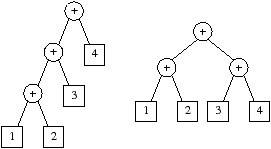
\includegraphics {drafts/book010}}
	\caption{\label{fig:basic_abstract_syntax_tree_examples}Абстрактные 
синтаксические деревья}
\end{figure}

Однако, структура дерева для $1 + 2$ одинакова в обоих случаях, поэтому мы 
можем его построить. В связи с тем что у нас отсутствует информация о части 
$+ 3$, мы временно сохраним это информацию до нужного момента.

При построении дабстрактного синтаксического дерева мы воспользуемся стековым 
автоматом, схожий с тем, который используется {\it yacc} (см. \ref{??}). 
Лексему читаются одна за другой и помещаются в стек до тех пор, пока у нас не 
будет достаточно информации, чтобы построить выражение. После этого, лексемы 
удаляются из стека и заменяются построенным выражением. Эта операция называется 
редукцией. 

Тип помещаемых в стек элементов следующий:

\begin{lstlisting}[language=OCaml]
# type exp_elem = 
     Texp of expression   (* expression         *)
   | Tbin of op_bin       (* opérateur binaire  *)
   | Tunr of op_unr       (* opérateur unaire   *)
   | Tpg                  (* parenthèse gauche  *) ;;
\end{lstlisting}

Заметим, что правые скобки не сохраняются, так как лишь левые скобки важны при 
операции редукции.

На рисунке \ref{fig:basic_abstract_syntax_tree_construction_example} 
проиллюстрировано изменение стека при анализе выражения $(1 + 2 * 3) * 4$. 
Символ над стрелкой есть текущий символ строки.

\begin{figure}[h]
	\center{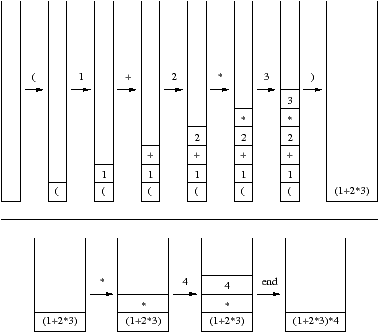
\includegraphics {drafts/book011}}
	\caption{\label{fig:basic_abstract_syntax_tree_construction_example}Basic: 
Пример создания абстрактного синтаксического дерева}
\end{figure}

Определим исключение для синтаксических ошибок.

\begin{lstlisting}[language=OCaml]
# exception ParseError ;;
\end{lstlisting}

Сначала определим операторы при помощи символов.

\begin{lstlisting}[language=OCaml]
# let symb_unr = function 
   "!" -> NON | "-" -> OPPOSE | _ -> raise ParseErreur 
 let symb_bin = function
     "+" -> PLUS | "-" -> MOINS | "*" -> MULT | "/" -> DIV | "%" -> MOD 
   | "=" -> EGAL | "<" -> INF | "<=" -> INFEQ | ">" -> SUP 
   | ">=" -> SUPEQ | "<>" -> DIFF | "&" -> ET | "|" -> OU 
   | _ -> raise ParseErreur 
 let tsymb s = try Tbin (symb_bin s) with ParseErreur -> Tunr (symb_unr s) ;;
val symb_unr : string -> op_unr = <fun>
val symb_bin : string -> op_bin = <fun>
val tsymb : string -> exp_elem = <fun>
\end{lstlisting}

Функция \code{reduce} реализует редукцию стека. Существует два случая, в 
которых стек начинается:

\begin{itemize}
	\item выражение, с последующим унарным оператором

	\item выражение, затем бинарный оператор и другое выражение. 
\end{itemize}

Кроме того, другой аргумент функции \code{reduce} --- это минимальный 
приоритет, который должен иметь оператор, чтобы редукция имела место. Для 
приведения без условий достаточно указать минимальный нулевой приоритет.

\begin{lstlisting}[language=OCaml]
# let reduce pr = function 
     (Texp e)::(Tunr op)::st  when  (priority_uop op) >= pr
        -> (Texp (ExpUnr (op,e)))::st
   | (Texp e1)::(Tbin op)::(Texp e2)::st  when  (priority_binop op) >= pr
        -> (Texp (ExpBin (e2,op,e1)))::st 
   | _ -> raise ParseError ;;
val reduce : int -> exp_elem list -> exp_elem list = <fun>
\end{lstlisting}

Заметим, что элементы выражения помещаются в стек в порядке чтения, из--за чего 
необходимо поменять местами операнды бинарной операции.

\code{stack\_or\_reduce} это главная функция синтаксического анализа, в 
соответствии с переданной ей лексемой она либо помещает новый элемент в стек 
либо выполняет редукцию.

\begin{lstlisting}[language=OCaml]
# let rec stack_or_reduce lex stack = match lex , stack with 
     Lint n ,  _      ->  (Texp (ExpInt n))::stack 
   | Lident v ,  _    ->  (Texp (ExpVar v))::stack 
   | Lstring s , _    ->  (Texp (ExpStr s))::stack
   | Lsymbol "(" , _  ->  Tlp::stack
   | Lsymbol ")" , (Texp e)::Tlp::st  ->  (Texp e)::st
   | Lsymbol ")" , _ -> stack_or_reduce lex (reduce 0 stack) 
   | Lsymbol s , _ 
        -> let symbol = 
             if s<>"-" then tsymb s 
             (* remove the ambiguity of the ``-'' symbol           *)
             (* according to the last exp element put on the stack *)
             else match stack 
                  with (Texp _)::_  ->  Tbin MINUS 
                                | _ ->  Tunr UMINUS 
           in ( match symbol with 
                  Tunr op  ->  (Tunr op)::stack 
                | Tbin op  -> 
                    ( try stack_or_reduce lex (reduce (priority_binop op) 
                                               stack )
                      with ParseError -> (Tbin op)::stack )
                | _ -> raise ParseError )
   | _ , _ -> raise ParseError ;;
val stack_or_reduce : lexeme -> exp_elem list -> exp_elem list = <fun>
\end{lstlisting}

После того как все лексемы извлечены и помещены в стек, дерево абстрактного 
синтаксиса может быть построено из элементов оставшихся в стеке --- это задача 
функции \code{reduce\_all}. Если анализируемое выражение было правильно 
сформировано, то в стеке должен остаться лишь один элемент, содержащий дерево 
этого выражения.

\begin{lstlisting}[language=OCaml]
# let rec reduce_all = function
   | [] -> raise ParseError
   | [Texp x] -> x 
   | st -> reduce_all (reduce 0 st) ;;
val reduce_all : exp_elem list -> expression = <fun>
\end{lstlisting}

Основной функцией анализа выражений является \code{parse\_exp}. Она 
просматривает строку, извлекает различные лексемы и передаёт их функции 
\code{stack\_or\_reduce}. Анализ прекращается, когда текущая лексема 
соответствует предикату переданному в аргументе.

\begin{lstlisting}[language=OCaml]
# let parse_exp stop cl = 
   let p = ref 0 in 
   let rec parse_one stack  = 
     let l = ( p:=cl.current ; lexer cl)
     in if not (stop l) then parse_one (stack_or_reduce l stack)
        else ( cl.current <- !p ; reduce_all stack )
   in parse_one []  ;;
val parse_exp : (lexeme -> bool) -> string_lexer -> expression = <fun>
\end{lstlisting}

Заметим, что лексема, которая определяет конец анализа, не используется при 
построении выражения. Для того чтобы проанализировать эту лексему позднее, 
необходимо установить текущую позицию на её начало (переменная \code{p}).

Перейдём теперь к анализу строки с инструкцией.

\begin{lstlisting}[language=OCaml]
# let parse_cmd cl = match lexer cl with 
     Lident s -> ( match s with 
         "REM" -> Rem (extract (fun _ -> true) cl)
       | "GOTO" -> Goto (match lexer cl with 
                           Lint p -> p 
                         | _ -> raise ParseError)
       | "INPUT" -> Input (match lexer cl with 
                             Lident v -> v 
                           | _ -> raise ParseError)
       | "PRINT" -> Print (parse_exp ((=) Lend) cl)
       | "LET" -> 
           let l2 = lexer cl and l3 = lexer cl 
           in ( match l2 ,l3 with 
                    (Lident v,Lsymbol "=") -> Let (v,parse_exp ((=) Lend) cl)
                  | _ -> raise ParseError )
       | "IF" -> 
           let test = parse_exp ((=) (Lident "THEN")) cl 
           in ( match ignore (lexer cl) ; lexer cl with 
                   Lint n  ->  If (test,n) 
                 | _ -> raise ParseError )
       | _ -> raise ParseError ) 
   | _ -> raise ParseError  ;;
val parse_cmd : string_lexer -> command = <fun>
\end{lstlisting}

И наконец, главная функция синтаксического анализа команд введённых 
пользователем в интерактивном цикле.

\begin{lstlisting}[language=OCaml]
# let parse str = 
   let cl = init_lex str 
   in match lexer cl with 
       Lint n -> Line { num=n ; cmd=parse_cmd cl }
     | Lident "LIST" -> List 
     | Lident "RUN" -> Run 
     | Lident "END" -> PEnd 
     | _ -> raise ParseError  ;;
val parse : string -> phrase = <fun>
\end{lstlisting}

\subsection{Вычисление}
\label{subsec:evaluation}

Программа на Basic состоит из набора строк и выполнение начинается с первой 
строки. Интерпретация строки программы заключается в исполнении задачи 
инструкции, которая находится на этой строке. Существует три множества 
инструкций: ввод/вывод ({\bf PRINT} и {\bf INPUT}), декларация переменных или 
присвоение ({\bf LET}) и переход ({\bf GOTO} и {\bf THEN}). Инструкции 
ввода/вывода реализуют взаимодействие с пользователем, для этого будут 
использованы соответствующие команды Objective CAML.

Для объявления и присвоения переменных, необходимо уметь вычислить значение 
арифметического выражение и знать расположение в памяти этой переменной. 
Результат вычисление выражения может быть либо целым числом, либо булевым 
значением, либо строкой. Сгруппируем их в типе \type{value}.

\begin{lstlisting}[language=OCaml]
# type value = Vint of int | Vstr of string | Vbool of bool  ;;
\end{lstlisting}

При объявлении переменной, нужно выделить память, чтобы хранить значение 
ассоциированное этой переменной. Для изменении переменной необходимо поменять 
значение связанно с именем переменной. Соответственно, программа Basic 
использует окружение, которое хранит связки имя переменной---значение. Данное 
окружение представлено в виде списка из пар (имя, значение).

\begin{lstlisting}[language=OCaml]
# type environment = (string * value) list ;;
\end{lstlisting}

Для того чтобы получить содержимое переменной мы используем её имя. При 
изменении значения переменной, меняется соответствующая пара.

В инструкциях перехода, условного или безусловного, указывается номер строки на 
которой должно продолжится выполнение программы. По умолчанию --- это следующая 
строка. В связи с этим, необходимо запомнить номер текущей строки.

Список инструкций из которых состоит программа, редактируемая в интерактивном 
цикле, не подходит для эффективного выполнения программы. Действительно, для 
того чтобы реализовать переход (\code{If} и \code{Goto}) необходимо 
пересмотреть весь список инструкций, чтобы найти строку с нужным номером. Для 
того чтобы можно было напрямую перейти на нужную строку, достаточно заменить 
структуру списка на вектор. В данном случае при переходе будет использоваться не 
номер строки, а её индекс в векторе. В этом случае, перед запуском программы 
командой \code{RUN}, проделаем пре--обработку инструкций, называемую 
компоновкой (assembly). По некоторым причинам, которые будут объяснены в 
следующем параграфе, скомпонованная программа представлена вектором строк, а не 
инструкций.

\begin{lstlisting}[language=OCaml]
# type code = line array ;;
\end{lstlisting}

Как и для калькулятора из прошлых глав, вычислитель использует состояние, 
которое изменяется при каждом вычислении. Информация, которую необходимо знать в 
каждый момент --- это программа в целом, следующая строка на выполнение и 
значения переменных. Выполняемая программа отличается от программы набранной в 
интерактивном цикле. Вместо того списка инструкций, мы используем вектор 
инструкций. Таким образом состояние программы описывается следующим типом.

\begin{lstlisting}[language=OCaml]
# type state_exec = { line:int ; xprog:code ; xenv:environment } ;;
\end{lstlisting}

Ошибки могут возникнуть в двух следующих случаях: вычисление выражения и переход 
на несуществующую строку. Соответственно, нужно обработать эти оба случая, чтобы 
интерпретатор корректно останавливался и выводил сообщение об ошибке. Определим 
исключение, а также функцию, которая будет его возбуждать и указывать номер 
строки на которой оно произошло.

\begin{lstlisting}[language=OCaml]
# exception RunError of int 
 let runerr n = raise (RunError n) ;;
exception RunError of int
val runerr : int -> 'a = <fun>
\end{lstlisting}

\subsection{Компоновка}
\label{subsubsec:assembly}

Компоновка программы, состоящей из списка нумерованных строк (тип 
\type{program}), заключается в переводе списка в вектор и корректировки 
инструкций перехода. Эта корректировка реализуется связкой номера строки и 
соответствующего ей индекса вектора. Для облегчения задачи, мы создаём вектор 
нумерованных строки. Данный вектор будет просматриваться каждый раз, когда 
необходимо найти индекс связанный со строкой. Если номер строки не найден, будет 
возвращено значение -1.

\begin{lstlisting}[language=OCaml]
# exception Result_lookup_index of int ;;
exception Result_lookup_index of int
# let lookup_index tprog num_line =
   try 
     for i=0 to (Array.length tprog)-1 do 
       let num_i = tprog.(i).num
       in if num_i=num_line then raise (Result_lookup_index i)
          else if num_i>num_line then raise (Result_lookup_index (-1))
     done ;
     (-1 )
   with Result_lookup_index i -> i ;;
val lookup_index : line array -> int -> int = <fun>

# let assemble prog =
   let tprog = Array.of_list prog in
     for i=0 to (Array.length tprog)-1 do
       match tprog.(i).cmd with
           Goto n -> let index = lookup_index tprog n
                     in tprog.(i) <- { tprog.(i) with cmd = Goto index }
         | If(c,n) -> let index = lookup_index tprog n
                      in tprog.(i) <- { tprog.(i) with cmd = If (c,index) }
         | _ -> ()
     done ;
   tprog ;;
val assemble : line list -> line array = <fun>
\end{lstlisting}

\subsection{Вычисление выражений}
\label{subsubsec:expression_evaluation}

Функция вычисления выражений обходит дерево абстрактного синтаксиса и выполняет 
операции, указанные в каждом узле дерева.

В следующих случаях возбуждается исключение \code{RunError}: несоответствие 
типов, деление на ноль и необъявленная переменная.

\begin{lstlisting}[language=OCaml]
# let rec eval_exp n envt expr = match expr with 
     ExpInt p  ->  Vint p
   | ExpVar v  -> ( try List.assoc v envt with Not_found -> runerr n )
   | ExpUnr (UMINUS,e) ->  
       ( match eval_exp n envt e with 
           Vint p -> Vint (-p) 
         | _ -> runerr n )
   | ExpUnr (NOT,e) ->  
       ( match eval_exp n envt e with 
           Vbool p -> Vbool (not p) 
         | _ -> runerr n )
   | ExpStr s -> Vstr s  
   | ExpBin (e1,op,e2) 
       -> match eval_exp n envt e1 , op , eval_exp n envt e2 with
               Vint v1 , PLUS   , Vint v2  ->  Vint (v1 + v2) 
             | Vint v1 , MINUS  , Vint v2  ->  Vint (v1 - v2) 
             | Vint v1 , MULT   , Vint v2  ->  Vint (v1 * v2) 
             | Vint v1 ,  DIV   , Vint v2  when v2<>0 ->  Vint (v1 / v2) 
             | Vint v1 ,  MOD   , Vint v2  when v2<>0 ->  Vint (v1 mod v2) 
 
             | Vint v1 , EQUAL   , Vint v2  ->  Vbool (v1 = v2) 
             | Vint v1 , DIFF    , Vint v2  ->  Vbool (v1 <> v2) 
             | Vint v1 ,  LESS   , Vint v2  ->  Vbool (v1 < v2) 
             | Vint v1 ,  GREAT  , Vint v2  ->  Vbool (v1 > v2) 
             | Vint v1 , LESSEQ  , Vint v2  ->  Vbool (v1 <= v2) 
             | Vint v1 , GREATEQ , Vint v2  ->  Vbool (v1 >= v2) 
 
             | Vbool v1 , AND , Vbool v2  ->  Vbool (v1 && v2) 
             | Vbool v1 , OR , Vbool v2  ->  Vbool (v1 || v2) 
 
             | Vstr v1 , PLUS , Vstr v2 -> Vstr (v1 ^ v2) 
             | _ , _ , _  -> runerr n  ;;
val eval_exp : int -> (string * value) list -> expression -> value = 
<fun>
\end{lstlisting}

\subsection{Вычисление инструкций}
\label{subsubsec:command_evaluation}

Для того, чтобы реализовать вычисление строки инструкций, нам понадобятся 
несколько дополнительных функций.

Добавление новой связки (имя переменной--значение) в окружение, заменяет 
старую, с таким же именем, если она существует.

\begin{lstlisting}[language=OCaml]
# let rec add v e env = match env with 
     [] -> [v,e]
   | (w,f)::l -> if w=v then (v,e)::l else (w,f)::(add v e l) ;;
val add : 'a -> 'b -> ('a * 'b) list -> ('a * 'b) list = <fun>
\end{lstlisting}

Другая функция, для вывода целых чисел или строк, пригодится при вычислении 
команды \code{PRINT}.

\begin{lstlisting}[language=OCaml]
# let print_value v = match v with 
     Vint n -> print_int n
   | Vbool true -> print_string "true"
   | Vbool false -> print_string "false"
   | Vstr s -> print_string s ;;
val print_value : value -> unit = <fun>
\end{lstlisting}

Вычисление инструкции есть переход из одного состояния в другое. В частности, 
окружение будет изменено, если инструкция это присвоение. Значение следующей 
строки на выполнение изменяется каждый раз. Если строка не существует, вернём 
значение -1.

\begin{lstlisting}[language=OCaml]
# let next_line state =
  let n = state.line+1 in
   if n < Array.length state.xprog then n else -1 ;;
val next_line : state_exec -> int = <fun>
# let eval_cmd state =
   match state.xprog.(state.line).cmd with 
     Rem _    ->  { state with line = next_line state }
   | Print e  ->  print_value (eval_exp state.line state.xenv e) ; 
                  print_newline () ;
                  { state with line = next_line state }
   | Let(v,e) ->  let ev = eval_exp state.line state.xenv e 
                    in { state with line = next_line state ; 
                                   xenv = add v ev state.xenv }
   | Goto n   ->  { state with line = n }
   | Input v  ->  let x = try read_int () 
                          with Failure "int_of_string" -> 0
                  in { state with line = next_line state; 
                                 xenv = add v (Vint x) state.xenv }
   | If (t,n) ->  match eval_exp state.line state.xenv t with 
                    Vbool true  -> { state with line = n }
                  | Vbool false -> { state with line = next_line state }
                  | _ -> runerr state.line  ;;
val eval_cmd : state_exec -> state_exec = <fun>
\end{lstlisting}

При каждом вызове функция перехода из одного состояние в другое 
\code{eval\_cmd} ищет текущую строку, выполняет её и затем устанавливает номер 
следующей строки как текущую строку. Если мы достигли последней строки 
программы, то номеру текущей строки присваивается значение -1, что позволит нам 
остановить программу.

\subsection{Вычисление программы}
\label{subsubsec:program_evaluation}

Будет рекурсивно применять функцию перехода, до тех пор, пока не получим 
состояние, в котором номер текущей строки равен -1.

\begin{lstlisting}[language=OCaml]
# let rec run state = 
  if state.line = -1 then state else run (eval_cmd state) ;;
val run : state_exec -> state_exec = <fun>
\end{lstlisting}

\subsection{Последние штрихи}
\label{subsec:finishing_touches}

Осталось лишь реализовать мини–редактор и собрать воедино все части программы, 
реализованные ранее.

Функция \code{insert} вставляет новую строку в соответствующее место в 
программе.

\begin{lstlisting}[language=OCaml]
# let rec insert line p = match p with  
     [] -> [line]
   | l::prog -> 
       if l.num < line.num then l::(insert line prog)
       else if l.num=line.num then line::prog
       else line::l::prog ;;
val insert : line -> line list -> line list = <fun>
\end{lstlisting}

Функция \code{print\_prog} выводит на экран код программы. 

\begin{lstlisting}[language=OCaml]
# let print_prog prog = 
   let print_line x = print_string (pp_line x) ; print_newline () in
    print_newline () ;
    List.iter print_line prog ;
    print_newline () ;;
val print_prog : line list -> unit = <fun>
\end{lstlisting}

Функция \code{one\_command} либо добавляет строку, либо выполняет команду. Она 
управляет состоянием интерактивного цикла, состоящего из программы и окружения. 
Это состояние, представленное типом \type{loop\_state}, отличается от состояние 
выполнения программы.

\begin{lstlisting}[language=OCaml]
# type loop_state = { prog:program; env:environment } ;;
# exception End ;;
\end{lstlisting}

\begin{lstlisting}[language=OCaml]
# let one_command state =
   print_string "> " ; flush stdout ;
   try 
     match parse (input_line stdin) with 
        Line l -> { state with prog = insert l state.prog }
      | List  -> (print_prog state.prog ; state )
      | Run 
       -> let tprog = assemble state.prog in
          let xstate = run { line = 0; xprog = tprog; xenv = state.env } in
           {state with env = xstate.xenv }
      | PEnd -> raise End
   with 
       LexerError -> print_string "Illegal character\n"; state 
     | ParseError -> print_string "syntax error\n"; state 
     | RunError n -> 
         print_string "runtime error at line ";
         print_int n ;
         print_string "\n";  
         state ;;
val one_command : loop_state -> loop_state = <fun>
\end{lstlisting}

Главной функцией является \code{go}, она запускает интерактивный цикл Basic.

\begin{lstlisting}[language=OCaml]
# let go () = 
 try 
   print_string "Mini-BASIC version 0.1\n\n";
   let rec loop state = loop (one_command state)  in 
     loop { prog = []; env = [] }
 with End -> print_string "See you later...\n";;
val go : unit -> unit = <fun>
\end{lstlisting}

Цикл реализуется локальной функцией \code{loop}. Цикл заканчивается при 
возбуждении исключения \code{End} функцией \code{one\_command}.

\subsection{Пример C+/C-}
\label{subsubsec:example_C_pm}

Вернёмся к игре C+/C-, описанной в \ref{subsec:Example_Higher_Lower}. Вот её 
эквивалент, написанный на Basic.

\begin{lstlisting}[language={[Visual]Basic}]
10 PRINT "Give the hidden number: "
20 INPUT N
30 PRINT "Give a number: "
40 INPUT R
50 IF R = N THEN 110
60 IF R < N THEN 90
70 PRINT "C-"
80 GOTO 30
90 PRINT "C+"
100 GOTO 30
110 PRINT "CONGRATULATIONS"
\end{lstlisting}

Пример запуска данной программы.

\begin{lstlisting}
> RUN
Give the hidden number:
64
Give a number:
88
C-
Give a number:
44
C+
Give a number:
64
CONGRATULATIONS
\end{lstlisting}

\subsection{Что дальше?}
\label{subsubsec:further_work}

Данный интерпретатор Basic обладает минимумом возможностей. Тем, кто желает его 
обогатить, мы предлагаем следующие расширения:

\begin{itemize}
	\item {\it числа с плавающей запятой}: наш интерпретатор распознает лишь 
целые числа, булевы значения и строки. Добавьте числа с плавающей запятой, а так 
же соответствующие операции в грамматику языка. Кроме лексического анализа, 
необходимо изменить вычисление с учётом приведения типов между целыми числами и 
числами с плавающей запятой.

	\item {\it векторы}: то есть добавить к синтаксису инструкцию \code{DIM 
var[x]}, при помощи который объявляется вектор \code{var} размером \code{x}. А 
так же выражение \code{var[i]}, которое ссылается на \code{i}--ый элемент 
вектора \code{var}.

	\item директивы: добавить директивы \code{SAVE "file\_name"} и \code{LOAD 
"file\_name"} для записи файла на диск и загрузки с диска соответственно.

	\item подпрограммы: вызов подпрограммы осуществляется инструкцией 
\code{GOSUB} номер строки. Эта инструкция реализует переход на этот номер и 
сохраняет при этом номер строки из которой произошёл вызов. Инструкция 
\code{RETURN} продолжает выполнение программы со строки, которая следует за 
последним вызовом \code{GOSUB}, если она существует, или выходит из программы. 
Для этого, вычисление должно контролировать не только окружение, но и стек, в 
котором хранятся адреса возврата различных вызовов \code{GOSUB}. При помощи 
инструкции \code{GOSUB} можно объявлять рекурсивные подпрограммы.
\end{itemize}
